\section{Introduction}
\label{sec:intro}

The field of video generation has rapidly transitioned from synthesizing blurry, single-shot clips to attempting complex, cinematic multi-shot narratives (Text-to-Multi-Shot Video, T2MSV). However, current evaluation methodologies remain deeply anchored in a single-shot mindset. Existing quality and consistency metrics, such as Fréchet Video Distance (FVD) or frame-wise CLIP similarity, evaluate generated videos holistically. In multi-shot environments, this holistic approach introduces a critical structural vulnerability: it inadvertently rewards generative models that produce entirely static, unchanging videos, even when those models are explicitly prompted to execute highly dynamic scene transitions. We define this pervasive failure phenomenon as the \textbf{Static Video Trap}. When a prompt sequence demands a narrative leap—for example, jumping from a "dense rainforest" to "deep outer space"—a model that stubbornly generates a continuous rainforest scene will score artificially high on traditional temporal consistency metrics. This creates the \textbf{Global Similarity Paradox}, where conventional metrics inherently reward the failure to transition, thereby masking the model's inability to follow complex shot-level semantic instructions.

\begin{figure}[t]
    \centering
    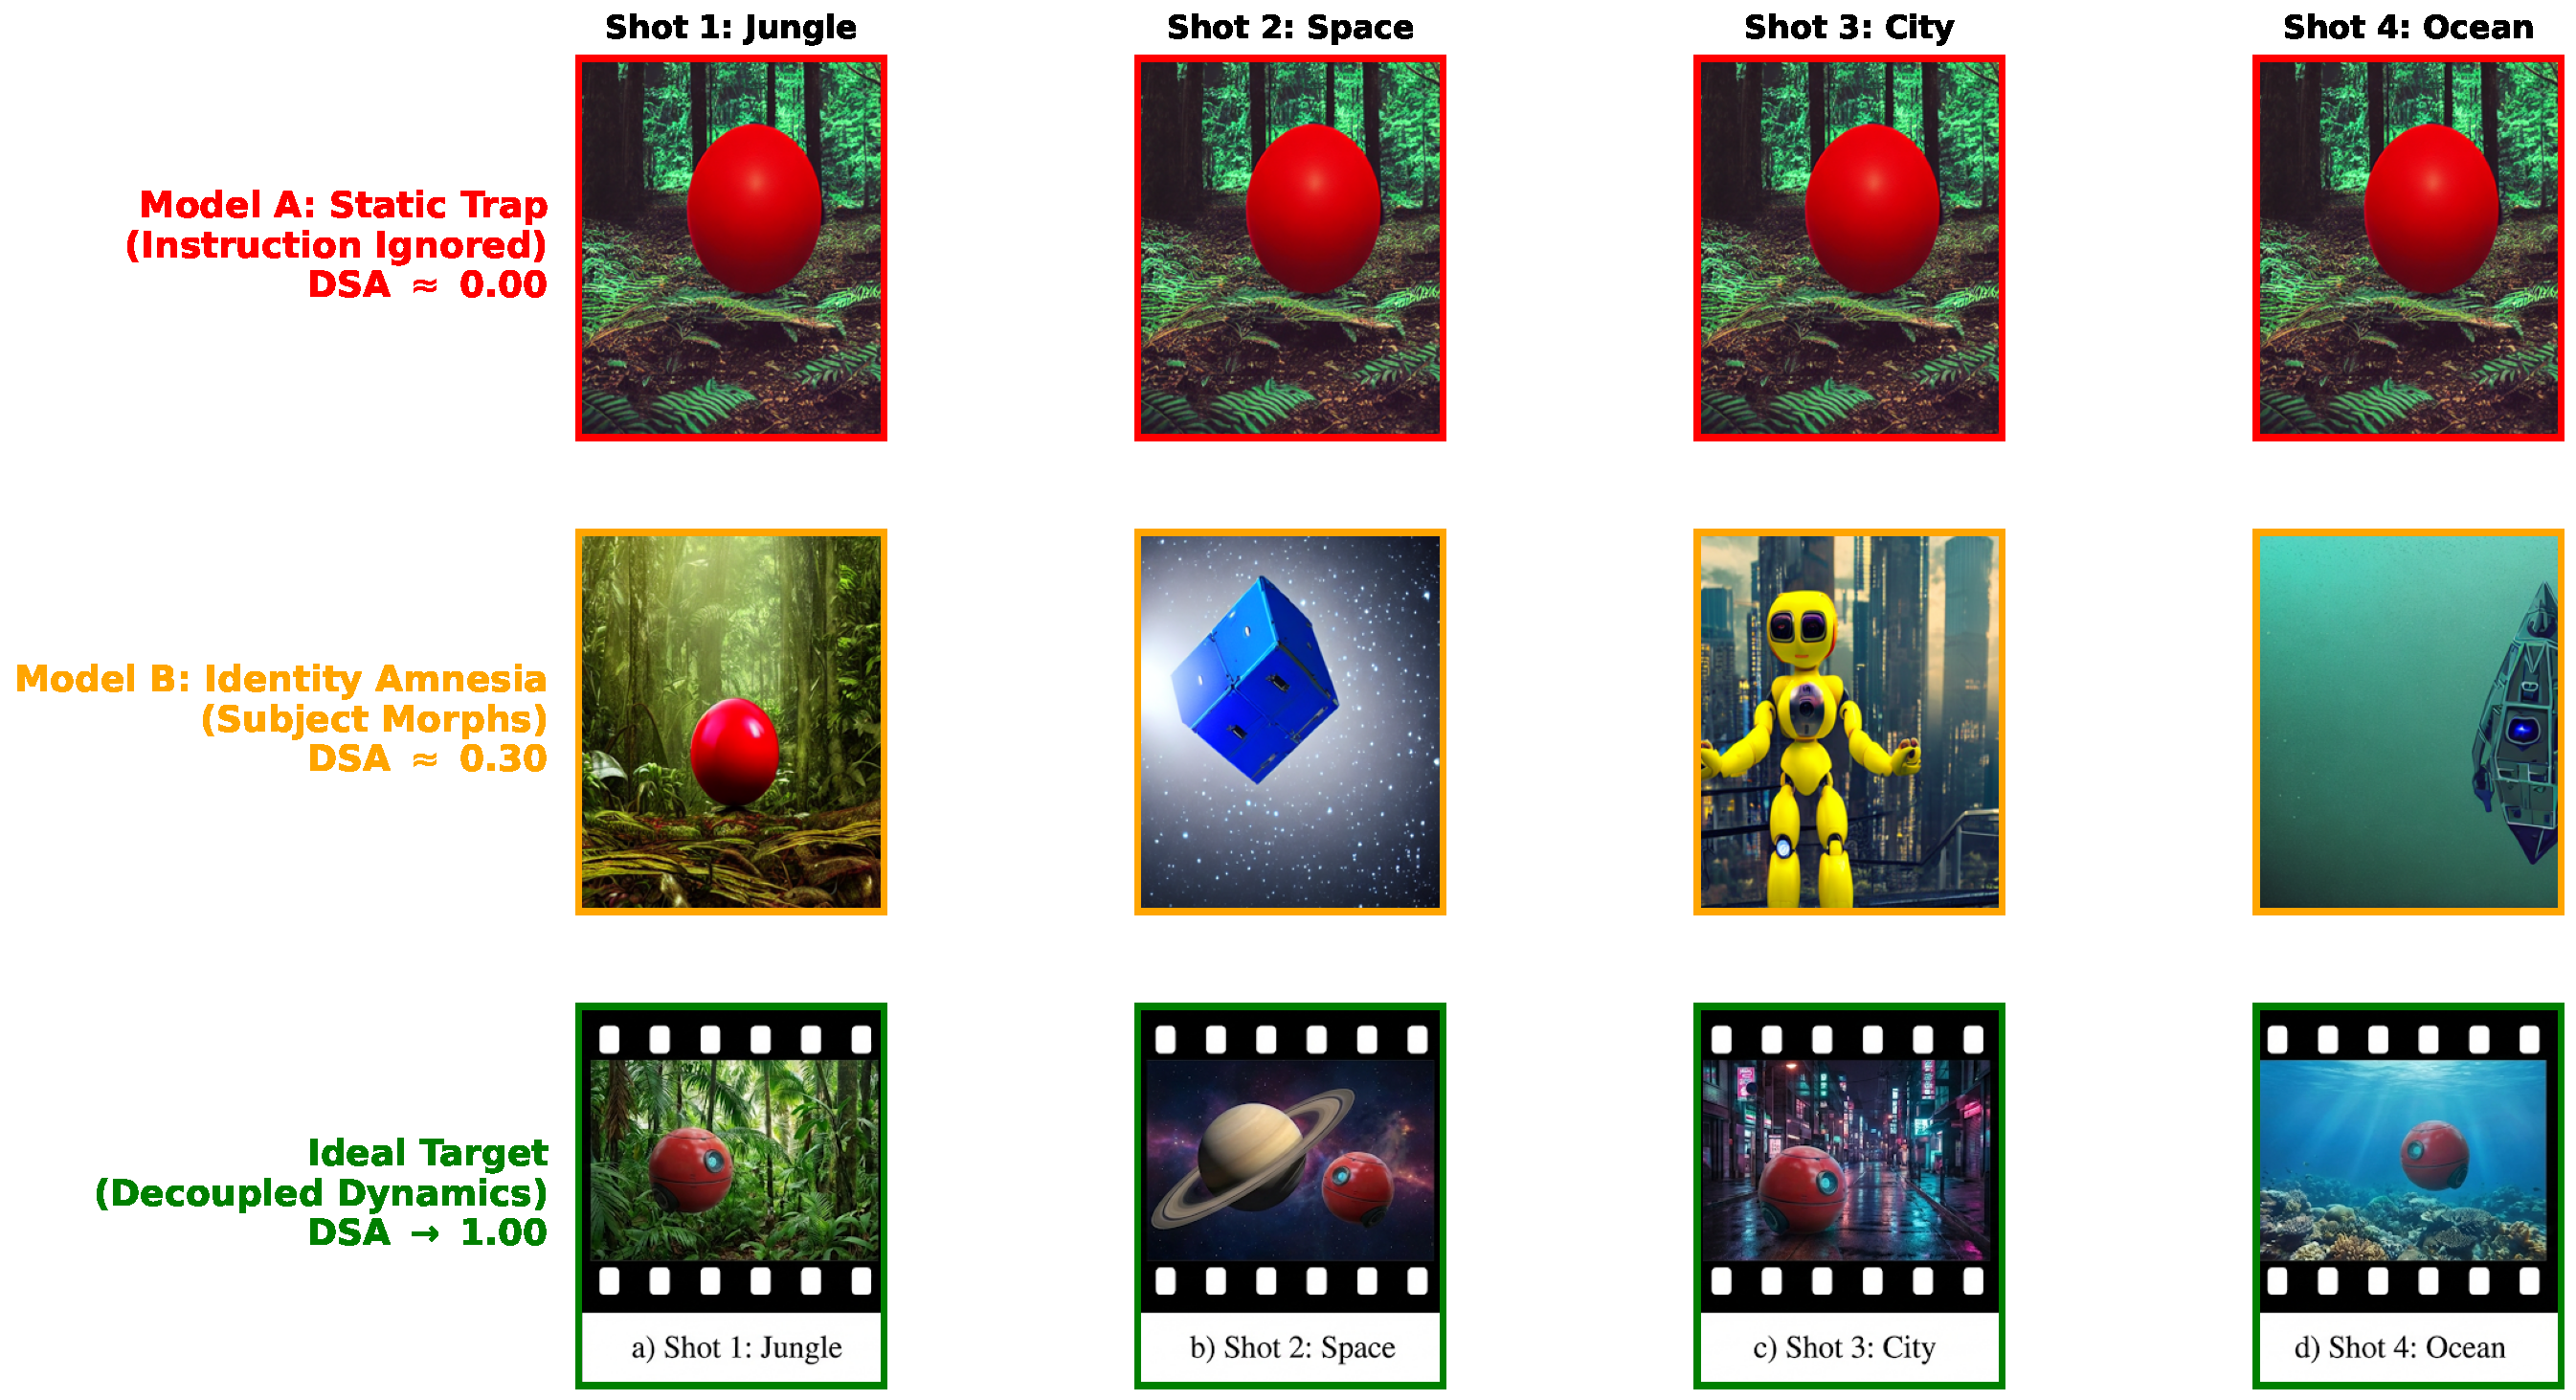
\includegraphics[width=\linewidth]{figures/fig1_teaser_robot.pdf}
    \caption{The dilemma of current T2MSV models illustrated with a "Retro-futuristic Robot" scenario. (A) \textbf{Static Trap}: The model (e.g., CogVideoX) maintains high temporal consistency by ignoring background change instructions, monotonously repeating the jungle environment across all shots. (B) \textbf{Identity Amnesia}: The model (e.g., StoryDiffusion) executes transitions but catastrophically fails to preserve the robot's specific geometry and color. (C) \textbf{Ideal Goal}: Our proposed benchmark demands both radical environmental dynamics and strict identity preservation.}
    \label{fig:teaser}
\end{figure}

Conversely, when advanced inference frameworks attempt to dynamically execute these semantic transitions to escape the static trap, they frequently succumb to \textbf{Identity Amnesia}, wherein the model loses the fine-grained visual features of the main subject across shots. In this work, we argue that evaluating T2MSV requires the precise quantitative management of \textit{intended discontinuities}. To address this, we introduce \textbf{Dynamic-MSV-Bench}, a comprehensive evaluation framework designed to rigorously disentangle subject identity preservation from environmental dynamics. Our benchmark categorizes evaluation into two orthogonal tracks. \textbf{Track S (Semantic Leap)} tests narrative diversity by requiring radical environment changes while strictly preserving the subject. In contrast, \textbf{Track M (Motion Continuity)} evaluates spatial integrity, where the background must remain perfectly consistent while the camera executes specific physical motions (e.g., panning or zooming). By cross-referencing performance across these two extremes, we establish a robust diagnostic taxonomy for generative failures.

To quantitatively support this taxonomy, we propose a 4D decoupled evaluation pipeline assessing subject identity, background dynamics, cut sharpness, and instruction alignment. Central to this pipeline is \textbf{Diagonal Semantic Alignment (DSA)}, a novel, mathematically rigorous metric that applies column-wise softmax normalization to shot-prompt similarity matrices. This explicitly assigns a strict zero score to static, instruction-ignoring videos, successfully neutralizing the Global Similarity Paradox.

Our core contributions are summarized as follows:
\begin{itemize}
    \item We empirically expose the \textbf{Static Trap} and \textbf{Identity Amnesia}, highlighting the fundamental flaws of legacy temporal metrics that inadvertently penalize intended cinematic cuts and semantic shifts.
    \item We introduce \textbf{Dynamic-MSV-Bench} alongside a 4D decoupled evaluation pipeline. This includes the mathematical formulation of \textbf{Diagonal Semantic Alignment (DSA)}, establishing a strict evaluation criterion for independent prompt adherence across multi-shot narratives.
    \item We conduct an exhaustive evaluation of state-of-the-art Foundation T2V models and specialized T2MSV frameworks, demonstrating that current monolithic architectures have not solved the underlying "Double-Kill" dilemma of multi-shot generation.
\end{itemize}